\documentclass{beamer}
\usetheme{Copenhagen}

\usepackage{fontspec}
\usepackage{enumerate}
\usepackage{amsmath,amsthm}
\usepackage{amsfonts}
\usepackage{amssymb}
\usepackage{pifont}
\usepackage{emoji}
\usepackage{biblatex}
\usepackage{textcomp}
\usepackage{MnSymbol}
\usepackage{caption}
\usepackage{fontawesome}

\usepackage{pdftexcmds}
\makeatletter
\let\pdfstrcmp\pdf@strcmp
\let\pdffilemoddate\pdf@filemoddate
\makeatother
\usepackage{svg}

\usepackage{tikz}
\usetikzlibrary{arrows, positioning}

\usepackage{parskip}
\usefonttheme{professionalfonts}
\usepackage{unicode-math}
\setmathfont{Latin Modern Math}

\usepackage{graphicx}
\usepackage{tikz}
\usepackage{tcolorbox}

% Define the logo and its position
\addtobeamertemplate{frametitle}{}{%
    \begin{tikzpicture}[remember picture,overlay]
        \node[anchor=north east, xshift=-3pt, yshift=-2pt] at (current page.north east) {
            
\includegraphics[height=0.6cm]{FU_LogoBajada_Blanco.png} % Adjust the height to make the logo smaller
        };
    \end{tikzpicture}%
}

\setbeamertemplate{itemize item}{\raisebox{-.05\height}{\small\ding{228}}}
\setbeamertemplate{itemize subitem}{--}
\setbeamertemplate{itemize subsubitem}{$\circ$}

\setbeamertemplate{enumerate item}[default]
\setbeamertemplate{enumerate subitem}[default]
\setbeamertemplate{enumerate subsubitem}[default]

\definecolor{color1}{RGB}{21,21,21}
\definecolor{blue}{RGB}{0,0,255}
\definecolor{grey}{RGB}{115, 117, 120}
\usecolortheme[named=color1]{structure}

\setsansfont{Archivo}[
    Path=./ArchivoFontFiles/,
    Scale=0.8,
    Extension = .ttf,
    UprightFont=*-Regular,
    BoldFont=*-SemiBold,
    ItalicFont=*-Italic,
    BoldItalicFont=*-BoldItalic
]

\usepackage{pst-node}
\usepackage{tikz-cd} 


\title{Introducción a la Inteligencia Artificial}
\author[Joan Gonzalez Quiroga\hspace{2mm}|\hspace{2mm}jgquiroga@dc.uba.ar]
{%
  \texorpdfstring{\centering
      {\large Joan Gonzalez Quiroga}\\
      {\footnotesize\href{mailto:jgquiroga@dc.uba.ar}{jgquiroga@dc.uba.ar}}
  }
  {Joan Gonzalez Quiroga}
}
\date{}

\begin{document}

\frame{\titlepage}

\begin{frame}
\frametitle{\textbf{Hoja de ruta}}

\begin{itemize}
    \item<1-> Introducción y relevancia histórica
    \item<2-> ¿Qué es un modelo? ¿Y uno generativo?
    \item<3-> Marco teórico: Neuronas artificiales y aprendizaje.
    \item<4-> Dimensión ética-social
    
\end{itemize}

\end{frame}

% DEFINICION ==========================================================================

\begin{frame}{\bfseries Definición}
\begin{center}
  \begin{tcolorbox}[width=0.8\textwidth]
    \raggedright
    {\itshape Definición -- }Llamamos \textbf{inteligencia artificial} al campo de la informática que se enfoca en desarrollar sistemas y programas capaces de realizar tareas que normalmente requieran \textit{`inteligencia humana'}.
  \end{tcolorbox}
\end{center}
\end{frame}

\begin{frame}{\bfseries Definición -- Mapa}
    \centering
    \raisebox{1\height}{
    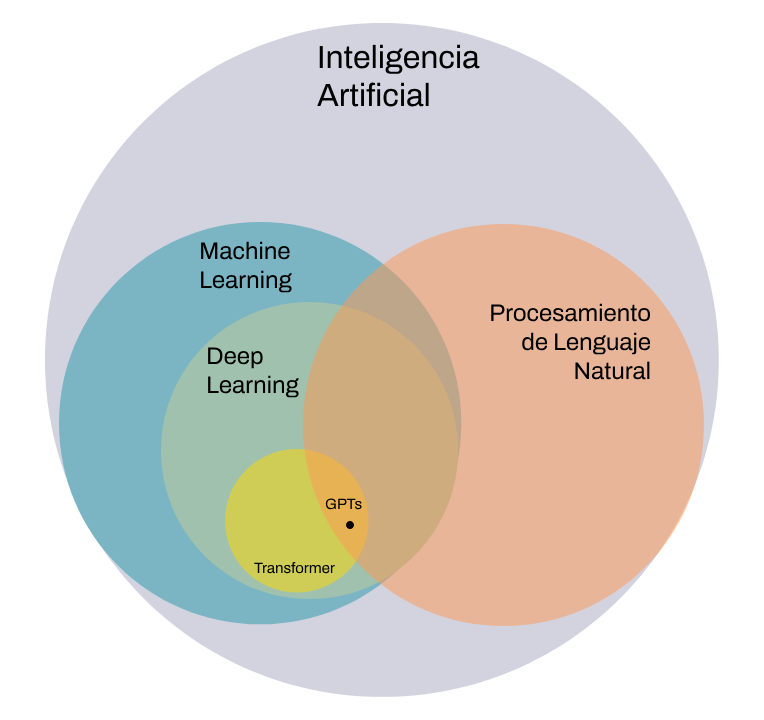
\includegraphics[height=7cm]{mapa-ia.png}
    }
\end{frame}

\begin{frame}{{\bfseries Definición}[es]}
\vspace{-5mm}
\begin{itemize}
    \item<1-> Inteligencia artificial {\color{grey}\textit{(en la tercer diapo!)}}
    \item<2-> \textit{Machine Learning}: Conjunto de técnicas que utilizan métodos estadísticos para identificar patrones en \textbf{grandes cantidades} de datos.
    \item<3-> Procesamiento de Lenguaje Natural (\textit{NLP}): Programas que manipulan, analizan, resumen o generan expresiones usando el lenguaje humano (coloquial, \textit{natural}) de manera automática.
    \item<4-> \textit{Deep Learning}: Un (sub)conjunto de métodos de \textit{machine learning} que surge de modelar el funcionamiento de las \textit{redes neuronales}. Se enfoca en intentar descubrir características, clasificaciones y representaciones `preexistentes' en los datos.
    \item<5-> \textit{Transformer}s: Arquitectura de \textit{deep learning}, diseñada para manipular {\color{grey}[una representación numérica de]} texto.
    \item<6-> \textit{GPT}: \textbf{G}enerative \textbf{P}retrained \textbf{T}ransformer (\textit{transformer} generativo pre-entrenado) \pause{\emoji{thumbs-up}}
\end{itemize}
\vspace{10mm}
\end{frame}

% Historia ============================================================================

\begin{frame}{\bfseries Brevísima historia de la Inteligencia Artificial}
 La idea de automatizar el razonamiento\footfullcite{Con distintas definiciones de `razonamiento' dependiendo del contexto} es tan antigua como la humanidad:
\begin{itemize}
    \item En Grecia (400$\sim$300 A.C.) apariciones mitológicas como \textit{Talos}. Pero también una de las primeras menciones sobre la `resolución de problemas como una búsqueda' (\textit{Means–ends analysis}) planteado por Aristóteles en \textit{Ethika Nikomacheia}.
    \item En el siglo XVII Hobbes escribe el Leviatán, donde aborda a la cognición como \textit{``nada más que un asunto de cálculos.''}. Algunos filósofos, como Descartes están en desacuerdo: \textit{``los fenómenos mentales tienen algo más, cierta \textbf{sustancia.}''}
\end{itemize}
\end{frame}

\begin{frame}{\bfseries Brevísima historia de la Inteligencia Artificial}
En el siglo XIX hay grandes avances y descubrimientos que profundizan el debate:
\begin{itemize}
    \item \textbf{Ada Lovelace} crea el primer \textit{programa} para la primer computadora, y cuestiona su capacidad de \textit{``simplemente hacer cálculos.''}
    \item \textbf{Bolazno} intenta por primera vez formalizar la \textit{semántica} -- el estudio lingüístico del significado de las palabras y símbolos.
    \item \textbf{Boole}, investigando \textit{``las leyes fundamentales de las operaciones mentales a través de las cuales razonamos, dándoles forma a través del lenguaje simbólico''} concluye inventando el \textbf{Álgebra de Boole}.
\end{itemize}
\end{frame}

\begin{frame}{\bfseries Brevísima historia de la Inteligencia Artificial}
\begin{itemize}
    \item En 1910 se muestra cómo todas las operaciones elementales de la matemática se pueden reducir a un razonamiento mecánico. (\textbf{Russel \& Whitehead}, \textit{Principia Mathematica}). Formalistas como \textbf{Hilbert} imaginan un sistema de deducción \textbf{automático} ...
    \item<2-> ... pero más tarde \textbf{Wittgenstein} y \textbf{Gödel} demuestran formalmente la imposibilidad de dicha automatización.
\end{itemize}
\end{frame}

\begin{frame}
    \frametitle{[no tan] \bfseries Brevísima historia de la Inteligencia Artificial}

    \begin{columns}
        \begin{column}{0.4\textwidth}
            \centering
            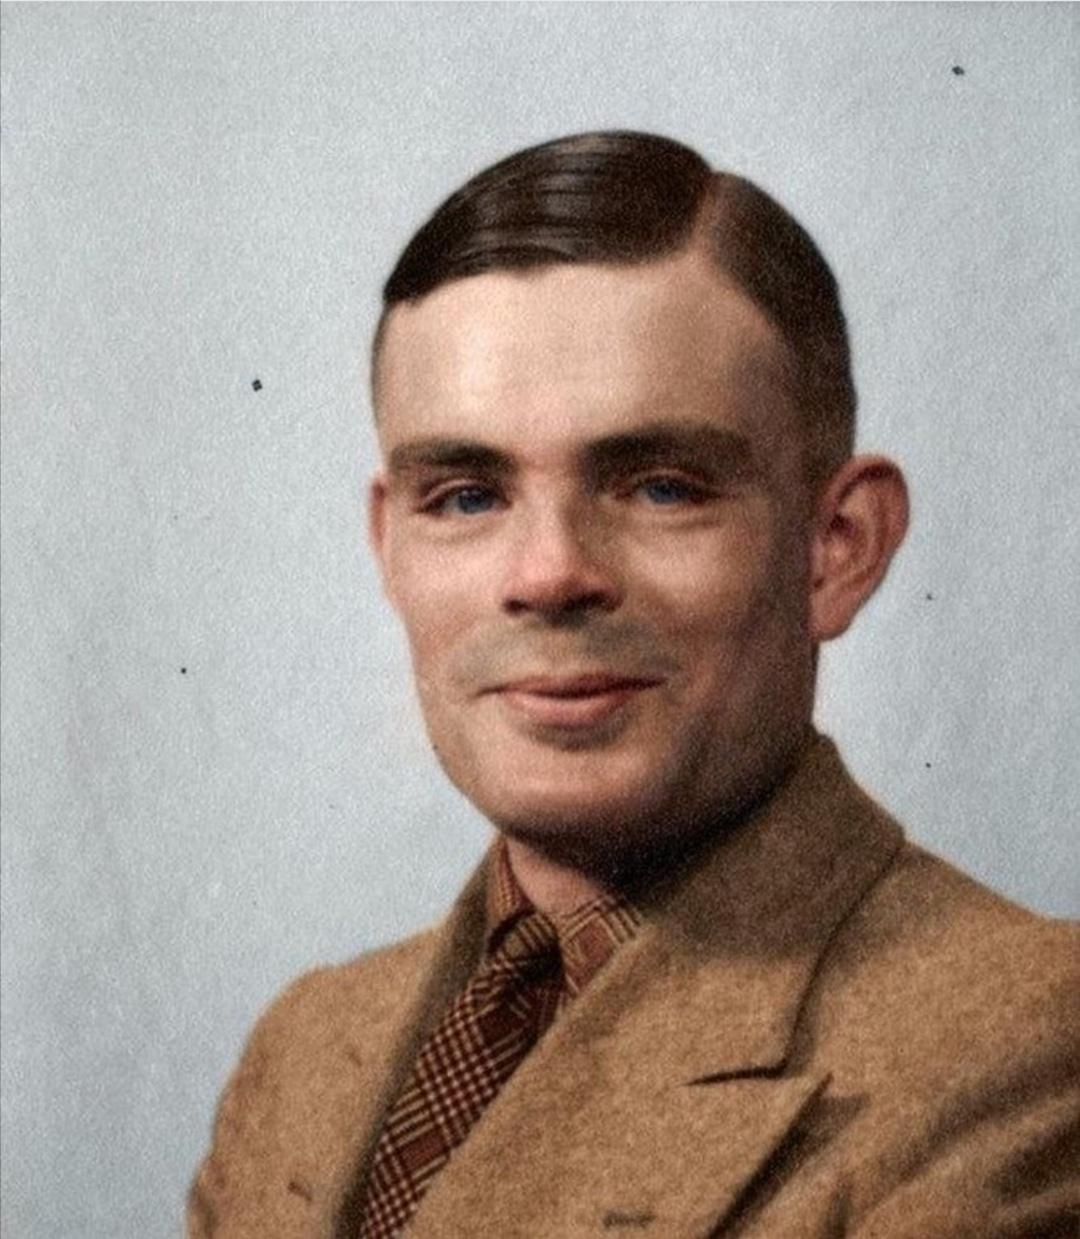
\includegraphics[width=\textwidth]{alan-turing-colorized.jpg}
            \pause
            \text{\footnotesize Foto colorizada por \@madsmadsen.ch}
            \text{\footnotesize Alan Turing, 1927.}\\
        \end{column}
        
        \begin{column}{0.6\textwidth}
        \textbf{Alan Turing}, considerado el padre de la Computación (y a veces también de la Inteligencia Artificial), publicó en 1950 un trabajo fundacional del campo titulado \textit{``Computing Machinery and Intelligence''}
        que comienza planteándose: \textbf{¿Pueden las máquinas \textit{pensar}?} \par\vspace{1mm} El trabajo de Turing
        discute cómo resolver esta pregunta y propone un procedimiento al que llama ``el juego de la
        imitación'', hoy conocido como Test de Turing.
        \end{column}
        
    \end{columns}
\end{frame}

\begin{frame}{\texttt{No soy un robot}}

\centering
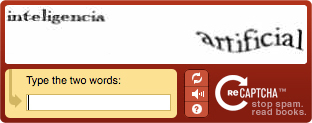
\includegraphics[width=5cm]{fake-captcha.jpg} \\
\pause
\vspace{10mm}
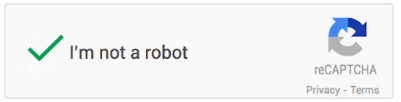
\includegraphics[width=5cm]{re-captcha.png} \\

\end{frame}

\begin{frame}
    \frametitle{\texttt{No soy un robot}}

    \begin{columns}
        \begin{column}{0.4\textwidth}
            \centering
            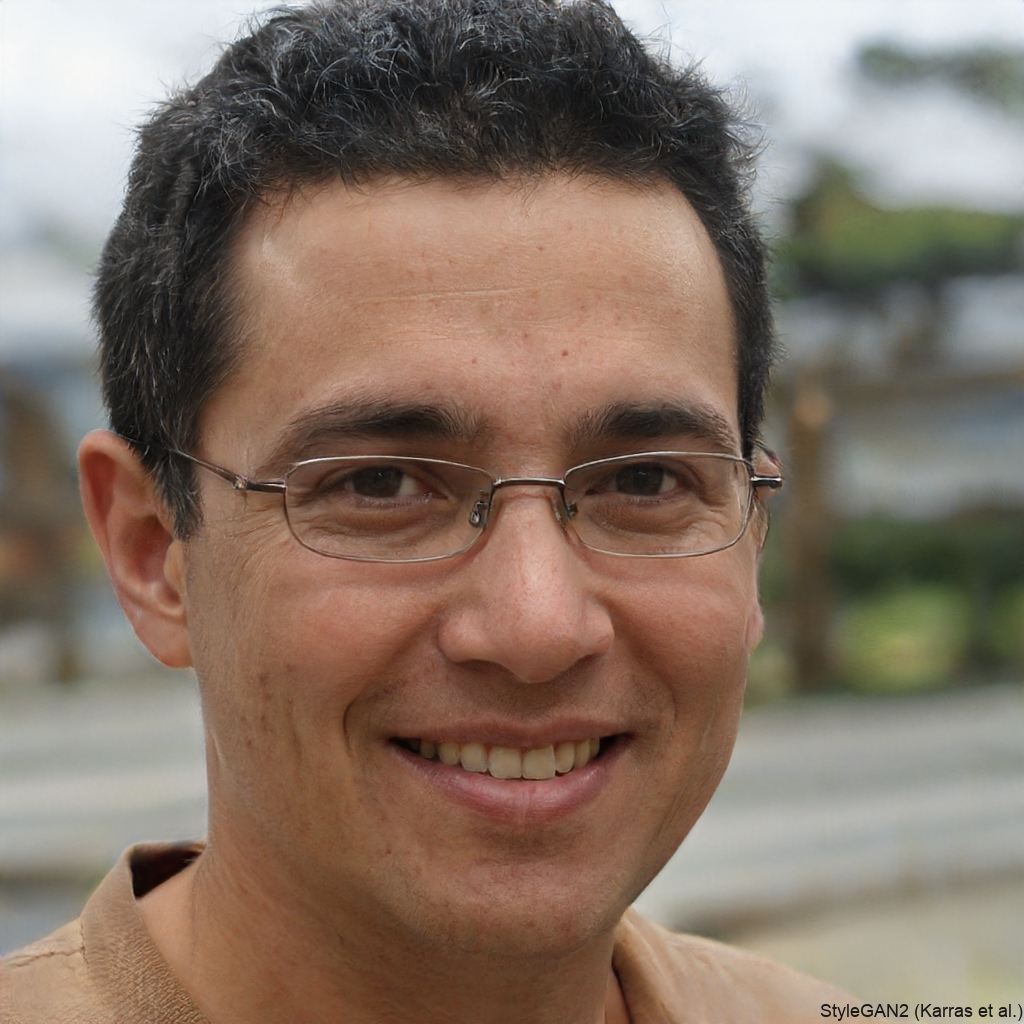
\includegraphics[width=\textwidth]{thispersondoesnotexist.png}
            \text{\footnotesize \phantom{thispersondoesnotexist.com}}
            \text{\footnotesize \phantom{¡Esta persona no existe!}}
            \end{column}
        \begin{column}{0.6\textwidth}
        \end{column}
    \end{columns}
\end{frame}

% Que es un modelo? =================================================================

\begin{frame}{\texttt{No, soy un robot!}}
        \begin{columns}
        \begin{column}{0.4\textwidth}
            \centering
            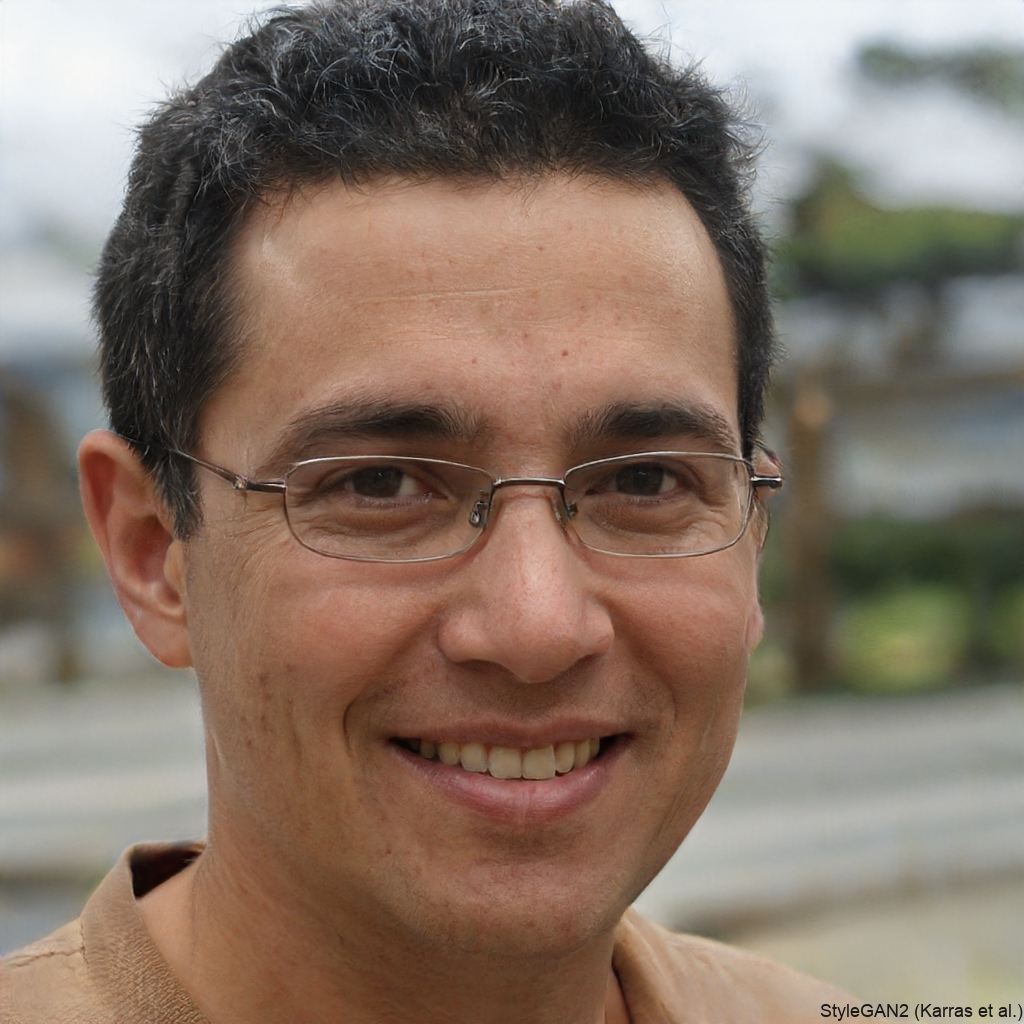
\includegraphics[width=\textwidth]{thispersondoesnotexist.png}
            \text{\footnotesize thispersondoesnotexist.com}
            \text{\footnotesize ¡Esta persona no existe!}\\
        \end{column}
        \begin{column}{0.6\textwidth}
        \textbf{El presente: } Modelos generativos
        \begin{itemize}
            \item ¿Qué es un \textit{modelo}?
            \item ¿Qué es un \textit{modelo generativo}?
        \end{itemize}
        \end{column}
        \end{columns}
\end{frame}

\begin{frame}{\textbf{¿Qué es un modelo?}}
    La palabra \textit{modelo} tiene distintos significados en distintas áreas de la ciencia y tecnología. A fines de simplificar la explicación, tomemos la siguiente definición:\par\vspace{1mm}
    \centering
    \begin{tcolorbox}[width=0.8\textwidth]
    \raggedright
    Llamamos \textbf{modelo} a alguna representación que describe algún fenómeno observable. Un \textbf{modelo matemático} es una definición concreta y concisa de dicha representación. Un \textbf{modelo de \textit{machine learning}} es un tipo de modelo matemático que tiene como objetivo representar el proceso de reconocer patrones en alguna cantidad de datos.
  \end{tcolorbox}
  \pause
  \textbf{No todos los modelos son matemáticos, no existe una sola forma de modelar, y no hay una única manera de hacer modelos de \textit{machine learning}.}
\end{frame}

\begin{frame}{\textbf{¿Qué es un modelo?}}

    \begin{figure}
        \centering
        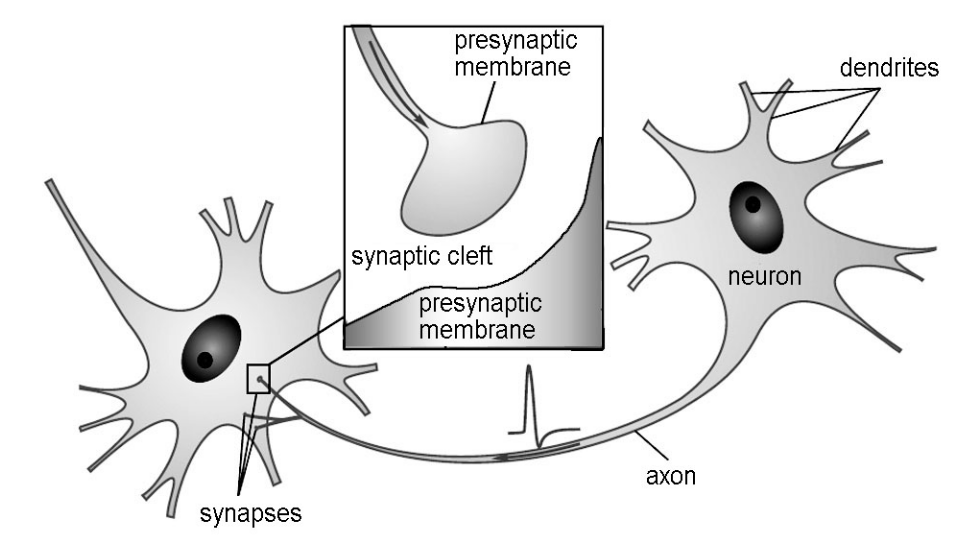
\includegraphics[width=0.75\linewidth]{neurona-esquematica.png}
        \captionsetup{labelformat=empty}
        \caption{Neurona Esquemática -- \textit{Nonlinear Dynamical Models of Neurons: Review}, A.S Dmitrichev et al.}
    \end{figure}
\end{frame}

\begin{frame}{\bfseries ¿Qué es un modelo?}
    \begin{figure}
        \centering
        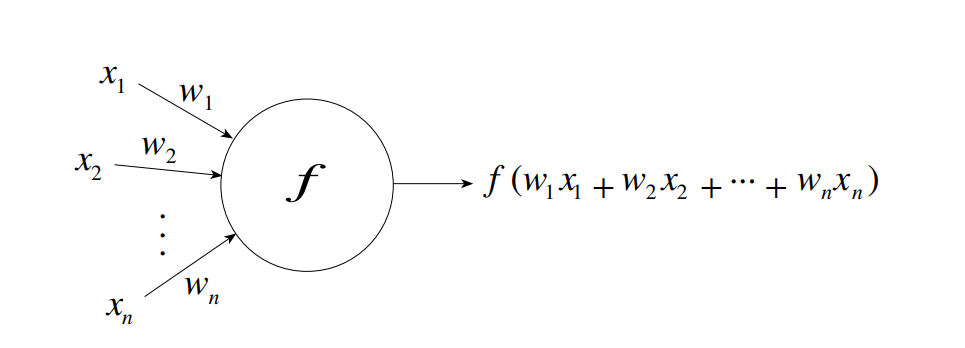
\includegraphics[width=0.75\linewidth]{perceptron.png}
        \captionsetup{labelformat=empty}
        \caption{Neurona Abstracta -- \textit{Neural Networks}, Raúl Rojas}
    \end{figure}
\end{frame}

\begin{frame}{\bfseries ¿Qué es un modelo?}
    \begin{figure}
        \centering
        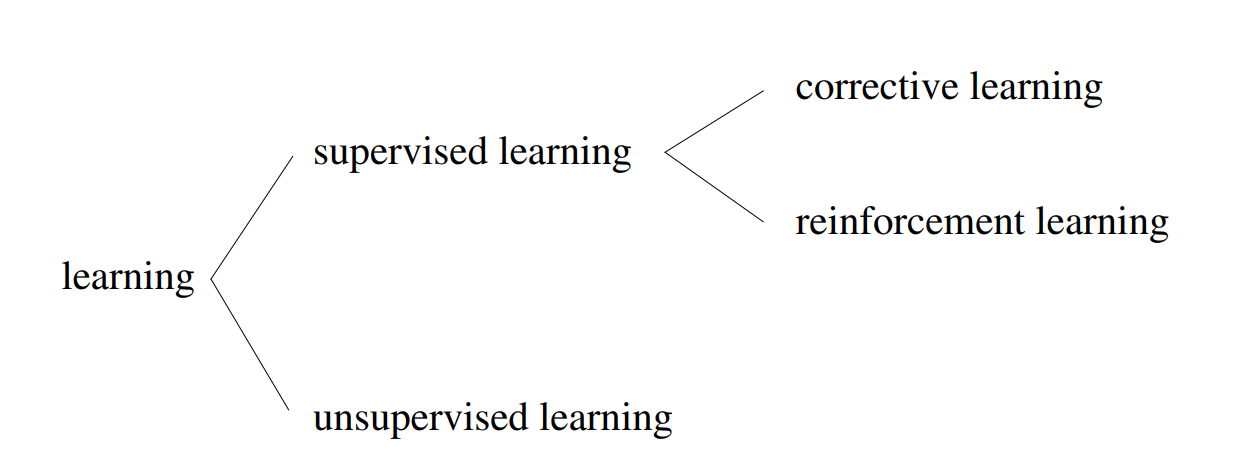
\includegraphics[width=0.75\linewidth]{learning.png}
        \captionsetup{labelformat=empty}
        \caption{Modelos de aprendizaje (automático) -- \textit{Neural Networks}, Raúl Rojas}
    \end{figure}
\end{frame}

\begin{frame}{\textbf{¿Qué es un modelo?}}

\begin{figure}[htbp]
    \centering
    \includesvg[width=\textwidth]{abs1.svg}
    \captionsetup{labelformat=empty}
    \caption{Hoare, 1972}
\end{figure}


\end{frame}

\begin{frame}{\textbf{¿Qué es un modelo?}}
\begin{figure}[htbp]
\centering
 \textit{"I started writing a program for a machine that did not exist, using a set of computer instructions that I dreamed up as they were needed"} \\
- Arthur Samuel, 1959
\end{figure}
\end{frame}

\begin{frame}{\bfseries Aspectos éticos-sociales}
\centering (Intencionalmente en blanco)
\end{frame}

\begin{frame}{\bfseries Aspectos sociales}
    \begin{figure}
        \centering
        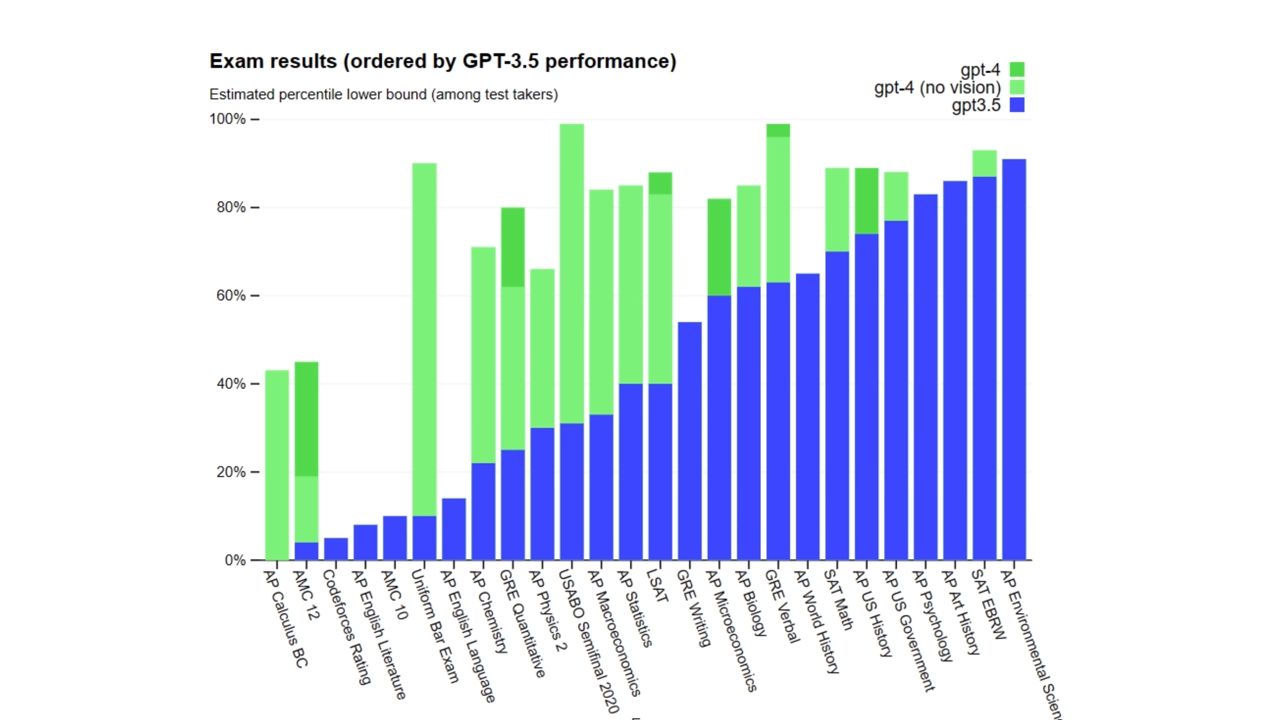
\includegraphics[width=1\linewidth]{tests-1.png}
        \captionsetup{labelformat=empty}
    \end{figure}
\end{frame}

\begin{frame}{\bfseries Aspectos sociales}
    \begin{figure}
        \centering
        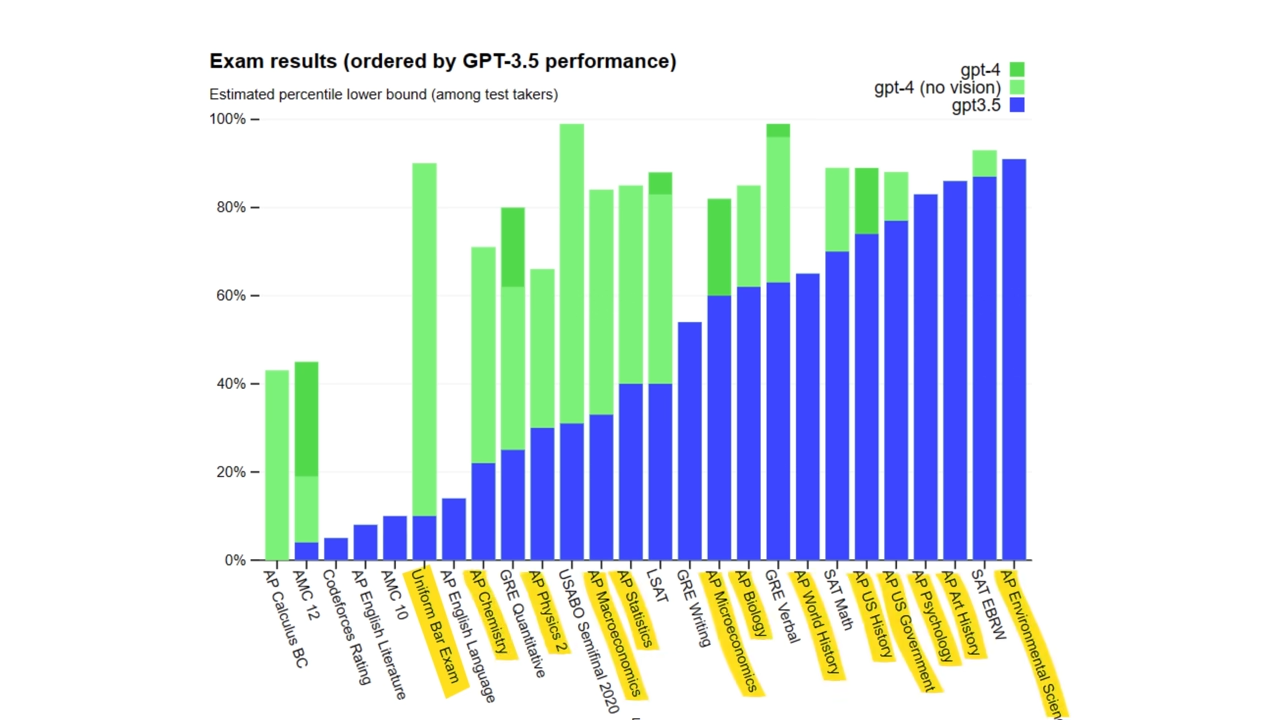
\includegraphics[width=1\linewidth]{tests-2.png}
        \captionsetup{labelformat=empty}
    \end{figure}
\end{frame}

\begin{frame}{\bfseries Aspectos sociales}
    \begin{figure}
        \centering
        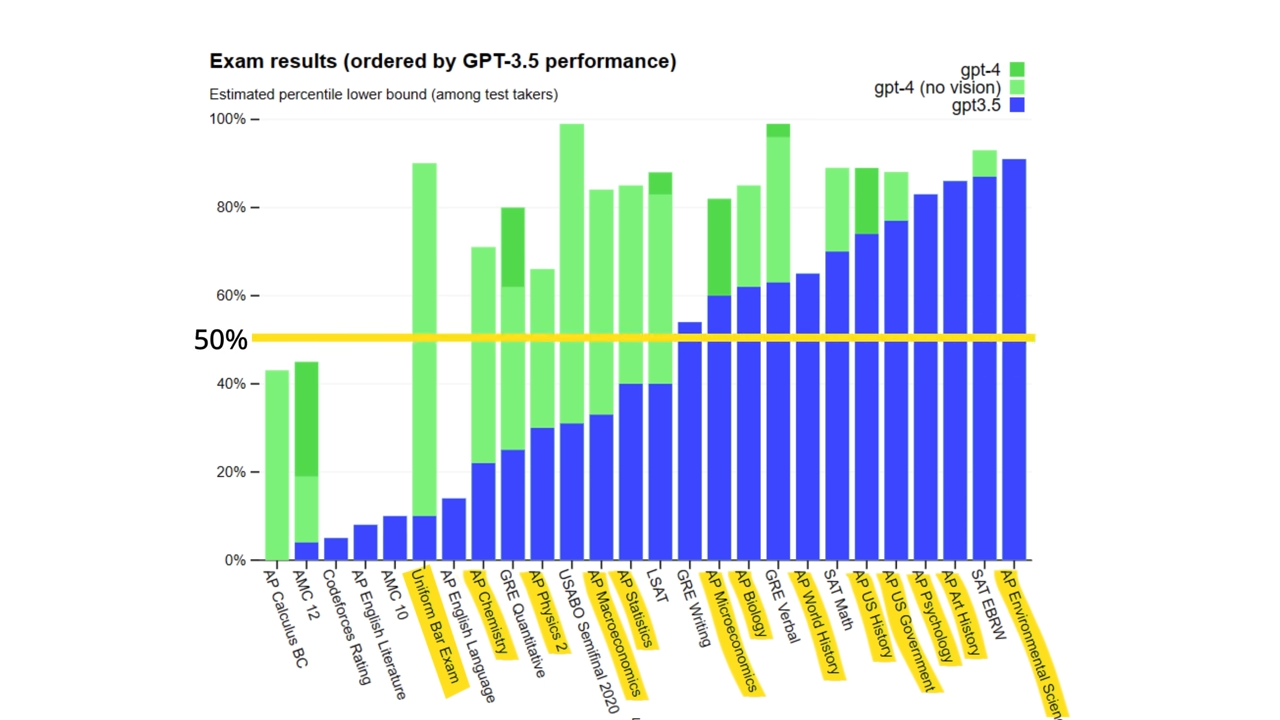
\includegraphics[width=1\linewidth]{tests-3.png}
        \captionsetup{labelformat=empty}
    \end{figure}
\end{frame}


%\centering\textbf{¡GeoGebra!} \\ 
%\href{https://www.geogebra.org/calculator/fzbmtqrw}{1}, %\href{https://www.geogebra.org/calculator/yednt7tn}{2}


% COMMUTATIVE DIAGRAM
% \begin{frame}{\phantom{}}
% 
%  \[ \psset{arrows=-T>, arrowinset=0.25, linewidth=0.6pt, nodesep=3pt, labelsep=2pt, rowsep=0.7cm, colsep = 1.1cm, shortput =tablr}
%  \everypsbox{\scriptstyle}
%  \begin{psmatrix}
%  A & B\\%
%  A_f & B_g
%  %%%
%  \ncline{1,1}{1,2}^{\varphi} \ncline{1,1}{2,1} <{\varrho_f }
%  \ncline{1,2}{2,2} > {\varrho_g}
%  \ncline{2,1}{2,2}^{\varphi_f}
%  \end{psmatrix}
%  \]
% 
% \end{frame}

\begin{frame}{\faGithub{}}
    \begin{figure}[h!]
    \centering
    
\includegraphics[width=0.5\textwidth]{qr.png}
    \vspace{-5mm}
    \captionsetup{labelformat=empty}
    \caption{\href{https://www.github.com/joangq/charla-iia}{github.com/joangq/charla-iia}}
\end{figure}

\end{frame}

\begin{frame}{\textbf{Bibliografía}}
    \begin{itemize}
        \item[\filledstar]\textit{Machines Who Think}, Pamela McCorduck
        \item[\filledstar]\textit{Neural Networks -- A Systematic Introduction}, Raúl Rojas
        \item[\filledstar]\textit{Artificial Intelligence: A Modern Approach}, Russel \& Norvig
        \item \textit{The Evolutionary Meaning of World -- Philosophy of the Social Sciences}, Hubert Cambier
        \item \textit{Tractatus Logico-Philosophicus}, Ludwig Wittgenstein
        \item \textit{A Logical Calculus of the Ideas Immanent in Nervous Activity}, McCulloch \& Pitts 
        \item \textit{Computing Machinery and Intelligence}, Alan Turing
        \item \textit{Minds, Machines and Gödel}, John R. Lucas
    \end{itemize}
\end{frame}

\end{document}